\documentclass[14pt,a4paper]{article}
\usepackage[14pt]{extsizes}
\usepackage[left=1.5cm, right=1.5cm, top=1.5cm, bottom=1.5cm]{geometry}
\usepackage[utf8]{inputenc}
\usepackage[T2A]{fontenc}
\usepackage[english, russian]{babel}
\usepackage{amsmath,amsfonts,amssymb,amsthm,mathtools} 
\usepackage{amsfonts}
\usepackage{amssymb}
\usepackage{titleps}
\usepackage{hyperref}
\usepackage{float}
\usepackage{graphicx}
\usepackage{multirow}
\usepackage{hhline}
\usepackage{wrapfig}
\usepackage{tikz}
\usepackage{pgfplots}
\usepackage{xcolor}
\usepackage{subfig}
\usepackage{upgreek}

\newcommand{\w}[1]{\text{#1}}
\newcommand{\und}[1]{\underline{#1}}
\newcommand{\img}[3]{
	\begin{figure}[H]
	\begin{center}
	\includegraphics[scale=#2]{#1}
	\end{center}
	\begin{center}
 	\textit{#3}
	\end{center}
	\end{figure}
}
\newcommand{\aw}[1]{
	\begin{center}
	\textit{#1}
	\end{center}
	\n
}
\newcommand{\be}[1]{
	\begin{center}
	\boxed{#1}
	\end{center}
}
\newcommand{\beb}[1]{
	\begin{equation}
	\boxed{#1}
	\end{equation}
}
\newcommand{\eb}[1]{
	\begin{equation}
	#1
	\end{equation}
}
\newcommand{\n}{\hfill \break}
\newcommand{\x}{\cdot}

\begin{document}
	\begin{center}
		{\large МОСКОВСКИЙ ФИЗИКО-ТЕХНИЧЕСКИЙ ИНСТИТУТ (НАЦИОНАЛЬНЫЙ ИССЛЕДОВАТЕЛЬСКИЙ УНИВЕРСИТЕТ)}
	\end{center}
	
	\vspace{4.5cm}
	{\huge
		\begin{center}
			{\bf Отчёт о выполнении лабораторной работы 3.6.1}\\
			Спектральный анализ электрических сигналов
		\end{center}
	}
	\vspace{2cm}
	\begin{flushright}
		{\LARGE Автор:\\ Киркича Андрей Александрович \\
			\vspace{0.2cm}
			Б01-202}
	\end{flushright}
	\vspace{3.2cm}
	\begin{center}
		Долгопрудный, 
		\today
	\end{center}
\n
\textbf{Цель работы: }
исследование резонанса токов в параллельном колебательном контуре с изменяемой ёмкостью, получение амплитудно-частотных и фазово-частотных характеристик, определение основных параметров контура.
	\n\n
	\textbf{В работе используются: }
	генератор сигналов произвольной формы, цифровой осциллограф с функцией быстрого преобразования Фурье.
	
%
%\subsection*{Разложение сложных сигналов на периодические колебания}
%В работе используется разложение в сумму синусов и косинусов с различными аргументами или, как чаще его называют, \textit{разложение в ряд Фурье}.
%\n\n
%Пусть задана функция $f(t)$, которая периодически повторяется с частотой $\Omega_1 = \dfrac{2\pi}{T}$, где $T$ --- период повторения импульсов. Её разложение в ряд Фурье имеет вид 
%\begin{equation}
%f(t) = \dfrac{a_0}{2} + \sum\limits_{n = 1}^{\infty}\left[a_n \cos \left(n \Omega_1t\right) + b_n \sin \left(n \Omega_1t\right)\right],
%\end{equation}
%\begin{equation}
%f(t) = \dfrac{a_0}{2} + \sum\limits_{n = 1}^{\infty}A_n \cos \left(n\Omega_1t-\psi_n\right).
%\end{equation}
%Если сигнал чётен относительно $t=0$, в тригонометрической записи остаются только члены с косинусами. Для нечетной - наоборот.
%\n\n
%Коэффициенты определяются по формуле:
%\begin{equation}
%\begin{array}{c}
%a_n  = \dfrac{2}{T}\int\limits_{t_1}^{t_1+T}f(t)\cos\left(n \Omega_1 t\right) dt, \ \ \
%b_n = \dfrac{2}{T}\int\limits_{t_1}^{t_1+T}f(t)\sin\left(n \Omega_1 t\right) dt.
%\end{array}
%\end{equation}
%\n
%Здесь $t_1$ --- время, с которого мы начинаем отсчет.
%\n\n
%Сравнив формулы $(1)$ и $(2)$, можно получить выражения для $A_n$  и $\psi_n$:
%\begin{center}
%    $A_n = \sqrt{a_n^2+b_n^2}, \ \ \ 
%    \psi_n = \arctg \dfrac{b_n}{a_n}.$
%\end{center}
%\subsection*{Периодическая последовательность прямоугольных импульсов}
%\begin{center}
%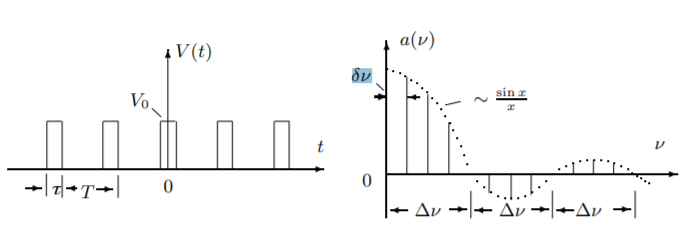
\includegraphics[scale=0.9]{pic1.png}
%\end{center}
%Введем величину: $\Omega_1 = \dfrac{2\pi}{T}$,
%где $T$ --- период повторения импульсов.
%\n\n
%Коэффициенты при косинусных составляющих будут равны
%\begin{center}
%    $a_n = \dfrac{2}{T}\int\limits_{-\tau/2}^{\tau/2}V_0\cos\left(n\Omega_1 t\right)dt = 2V_0\dfrac{\tau}{T}\dfrac{\sin\left(n\Omega_1\tau/2\right)}{n\Omega_1\tau/2} \sim \dfrac{\sin x}{x}.$
%\end{center}
%\n
%Здесь $V_0$ - амплитуда сигнала. Поскольку наша функция четная, то $b_n = 0$. Пусть $T$ кратно $\tau$. Тогда введем ширину спектра, равную $\Delta \omega$ --- расстояние от главного максимума до первого нуля огибающей, возникающего, как нетрудно убедиться при $n = \dfrac{2\pi}{\tau \Omega_1}$. При 
%этом
%\begin{center}
%    $\Delta \omega \tau \simeq 2\pi \Rightarrow \Delta \nu \Delta t \simeq 1.$
%\end{center}
%\subsection*{Периодическая последовательность цугов}
%\begin{center}
%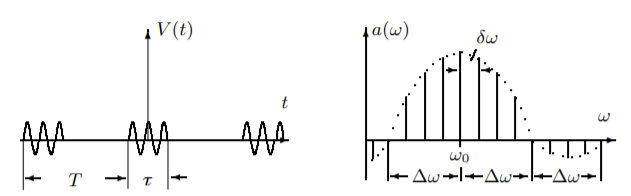
\includegraphics[scale=0.9]{pic2.png}
%\end{center}
%Возьмём цуги колебания $V_0 \cos(\omega_0 t)$ с длительностью цуга $\tau$ и периодом повторений $T$.\n\n
%Функция $f(t)$ снова является четной относительно $t = 0$. Коэффициент при $n$-ой гармонике согласно формуле $(3)$ равен
%\begin{center}
%    $a_n = \dfrac{2}{T}\int\limits_{-\tau/2}^{\tau/2}V_0 \cos \left(\omega_0t\right) \cdot \cos\left(n \Omega_1t\right)dt = V_0 \dfrac{\tau}{T}\left( \dfrac{\sin\left[\left(\omega_0 - n \Omega_1\right)\dfrac{\tau}{2}\right]}{\left( \omega_0 - n \Omega_1\right) \dfrac{\tau}{2}} + \dfrac{\sin\left[\left(\omega_0 + n \Omega_1\right)\dfrac{\tau}{2}\right]}{\left( \omega_0 + n \Omega_1\right) \dfrac{\tau}{2}}\right).$
%\end{center}
%Пусть $T$ кратно $\tau$. Тогда спектры последовательности прямоугильных сигналов и цугов аналогичны, но максимумы сдвинуты на $\omega_0$.
%\subsection*{Амплитудно-модулированные колебания}
%\begin{center}
%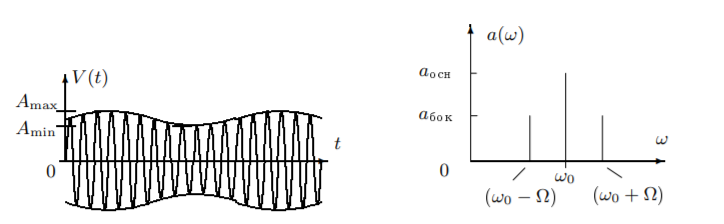
\includegraphics[scale=0.9]{pic3.png}
%\end{center}
%Рассмотрим гармонические колебания высокой частоты $\omega_0$, амплитуда которых медленно меняется по гармоническому закону с частотой $\Omega \ll \omega_0$:
%\begin{center}
%    $f(t) = A_0 \left[1+m\cos \Omega t\right] \cos \omega_0 t.$
%\end{center}
%Коэффициент $m$ называется \textit{глубиной модуляции}. При $m < 1$ амплитуда меняется от минимальной $A_{min} = A_0(1-m)$ до максимальной $A_{max} = A_0(1+m)$. Глубина модуляции может быть представлена в виде
%\begin{equation}
%m = \dfrac{A_{max}-A_{min}}{A_{max}+A_{min}}.
%\end{equation}
%Простым тригонометрическим преобразованием уравнения $(4)$ можно найти спектр колебаний:
%\begin{center}
%    $f(t) = A_0 \cos \omega_0t + \dfrac{A_0m}{2} \cos \left(\omega_0 + \Omega\right)t + \dfrac{A_0m}{2}\cos\left(\omega_0 - \Omega\right)t.$
%\end{center}

\section*{Теоретические сведения}

\subsection*{Разложение сложных сигналов на периодические колебания}
В работе используется разложение функции в сумму синусов и косинусов с различными аргументами или, как чаще его называют, \textit{разложение в ряд Фурье}.
\n\n
Пусть задана функция $f(t)$, которая периодически повторяется с частотой $\Omega_1 = \dfrac{2\pi}{T}$, где $T$ --- период повторения импульсов. Её разложение в ряд Фурье имеет вид: 
\begin{equation}
f(t) = \dfrac{a_0}{2} + \sum\limits_{n = 1}^{\infty}\left[a_n \cos \left(n \Omega_1t\right) + b_n \sin \left(n \Omega_1t\right)\right]
\end{equation}
или
\begin{equation}
f(t) = \dfrac{a_0}{2} + \sum\limits_{n = 1}^{\infty}A_n \cos \left(n\Omega_1t-\psi_n\right).
\end{equation}
Если сигнал чётен относительно $t=0$, в тригонометрической записи остаются только члены с косинусами. Для нечетного - наоборот.
\n\n
Коэффициенты определяются по формулам:
\begin{equation}
\begin{array}{c}
a_n  = \dfrac{2}{T}\int\limits_{t_1}^{t_1+T}f(t)\cos\left(n \Omega_1 t\right) dt,\\
\\
b_n = \dfrac{2}{T}\int\limits_{t_1}^{t_1+T}f(t)\sin\left(n \Omega_1 t\right) dt.
\end{array}
\end{equation}
Здесь $t_1$ --- время, с которого мы начинаем отсчет.
\n\n
Сравнив формулы $(1)$ и $(2)$, можно получить выражения для $A_n$  и $\psi_n$:
\begin{equation}
\begin{array}{l}
A_n = \sqrt{a_n^2+b_n^2},\\
 \psi_n = \arctan \dfrac{b_n}{a_n}.
\end{array}
\end{equation}
\subsection*{Периодическая последовательность прямоугольных импульсов}
\begin{center}
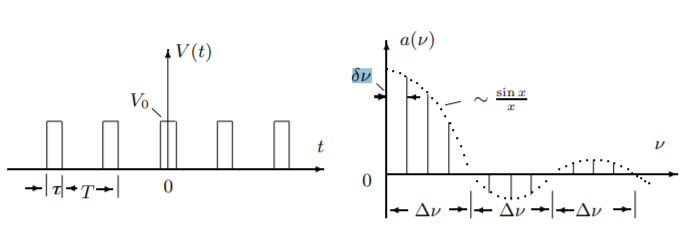
\includegraphics[scale=0.9]{2.png}
\end{center}
Введем величину: $\Omega_1 = \dfrac{2\pi}{T}$,
где $T$ --- период повторения импульсов.
\n\n
Коэффициенты при косинусных составляющих будут равны:
\begin{equation}
a_n = \dfrac{2}{T}\int\limits_{-\tau/2}^{\tau/2}V_0\cos\left(n\Omega_1 t\right)dt = 2V_0\dfrac{\tau}{T}\dfrac{\sin\left(n\Omega_1\tau/2\right)}{n\Omega_1\tau/2} \sim \dfrac{\sin x}{x}.
\end{equation}
\n
Здесь $V_0$ - амплитуда сигнала.
\n
Поскольку наша функция четная, $b_n = 0$. 
\n
Пусть $T$ кратно $\tau$. Тогда введем ширину спектра, равную $\Delta \omega$ --- расстоянию от главного максимума до первого нуля огибающей, возникающего, как нетрудно убедиться, при $n = \dfrac{2\pi}{\tau \Omega_1}$. При 
этом:
\begin{equation}
\Delta \omega \tau \simeq 2\pi \Rightarrow \Delta \nu \Delta t \simeq 1.
\end{equation}
\n В работе мы будем проверять справедливость этой формулы.
\subsection*{Периодическая последовательность цугов}
\begin{center}
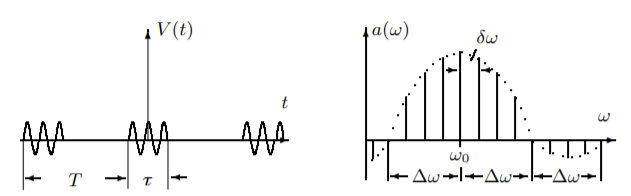
\includegraphics[scale=0.9]{3.png}
\end{center}
Возьмём цуги колебания $V_0 \cos(\omega_0 t)$ с длительностью цуга $\tau$ и периодом повторений $T$.\n\n
Функция $f(t)$ снова является четной относительно $t = 0$. Коэффициент при $n$-ой гармонике согласно формуле $(3)$ равен:
\begin{equation}
a_n = \dfrac{2}{T}\int\limits_{-\tau/2}^{\tau/2}V_0 \cos \left(\omega_0t\right) \cdot \cos\left(n \Omega_1t\right)dt = V_0 \dfrac{\tau}{T}\left( \dfrac{\sin\left[\left(\omega_0 - n \Omega_1\right)\dfrac{\tau}{2}\right]}{\left( \omega_0 - n \Omega_1\right) \dfrac{\tau}{2}} + \dfrac{\sin\left[\left(\omega_0 + n \Omega_1\right)\dfrac{\tau}{2}\right]}{\left( \omega_0 + n \Omega_1\right) \dfrac{\tau}{2}}\right).
\end{equation}
Пусть $T$ кратно $\tau$. Тогда спектры последовательности прямоугольных сигналов и цугов аналогичны, но максимумы сдвинуты на $\omega_0$.
\subsection*{Амплитудно-модулированные колебания}
\begin{center}
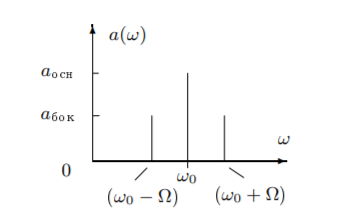
\includegraphics[scale=0.9]{4.png}
\end{center}
Рассмотрим гармонические колебания высокой частоты $\omega_0$, амплитуда которых медленно меняется по гармоническому закону с частотой $\Omega \ll \omega_0$:
\begin{equation}
f(t) = A_0 \left[1+m\cos \Omega t\right] \cos \omega_0 t.
\end{equation}
Коэффициент $m$ называется \textit{глубиной модуляции}. При $m < 1$ амплитуда меняется от минимальной $A_{min} = A_0(1-m)$ до максимальной $A_{max} = A_0(1+m)$. Глубина модуляции может быть представлена в виде
\begin{equation}
m = \dfrac{A_{max}-A_{min}}{A_{max}+A_{min}}.
\end{equation}
Простым тригонометрическим преобразованием уравнения $(8)$ можно найти спектр колебаний:
\begin{equation}
f(t) = A_0 \cos \omega_0t + \dfrac{A_0m}{2} \cos \left(\omega_0 + \Omega\right)t + \dfrac{A_0m}{2}\cos\left(\omega_0 - \Omega\right)t.
\end{equation}
\n
В дальнейшем мы будем использовать эту формулу.

\section*{Результаты измерений}

\subsection*{Исследование спектра периодических последовательностей прямоугольных импульсов}
Устанавив прямоугольные колебания c $\nu_{\text{повт}} = 1$ кГц (период $T = 1$ мс) и длительностью импульса $\tau = T/20 = 50$ мкс, мы получили на экране спектр сигнала и, изменяя либо $\tau$, либо $\nu_{\text{повт}}$, наблюдали, как изменяется спектр.
\begin{figure}[H]
    \centering
    \subfloat[$\nu_{\text{повт}} = 1$ кГц, $\tau = 50$ мкс]{{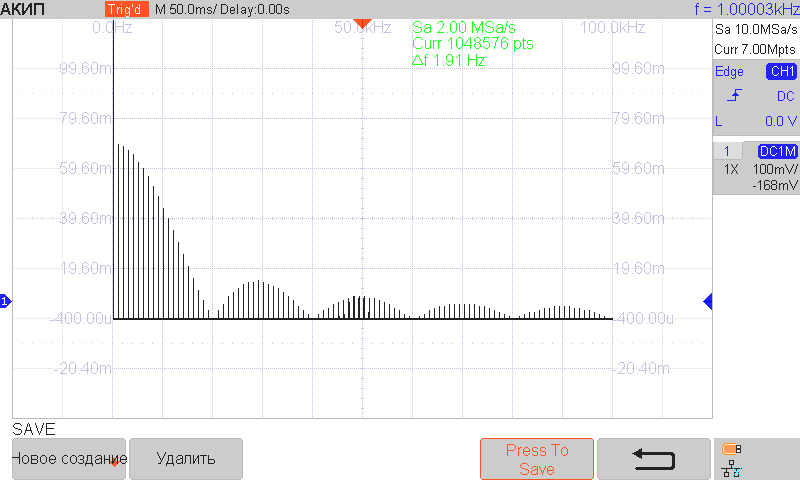
\includegraphics[width=0.5\textwidth]{AKIP0001.png}}}
    \subfloat[$\nu_{\text{повт}} = 1.5$ кГц, $\tau = 50$ мкс]{{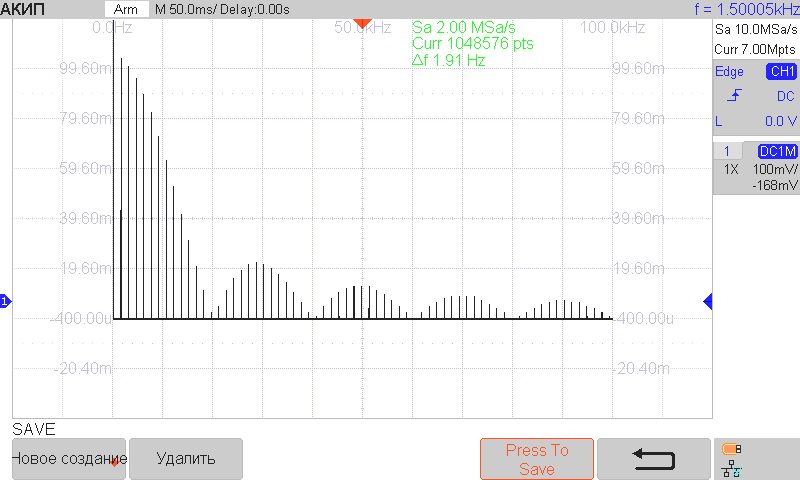
\includegraphics[width=0.5\textwidth]{AKIP0002.png}}}\\
    \end{figure}
\begin{figure}[H]
    \centering
    \subfloat[$\nu_{\text{повт}} = 2$ кГц, $\tau = 50$ мкс]{{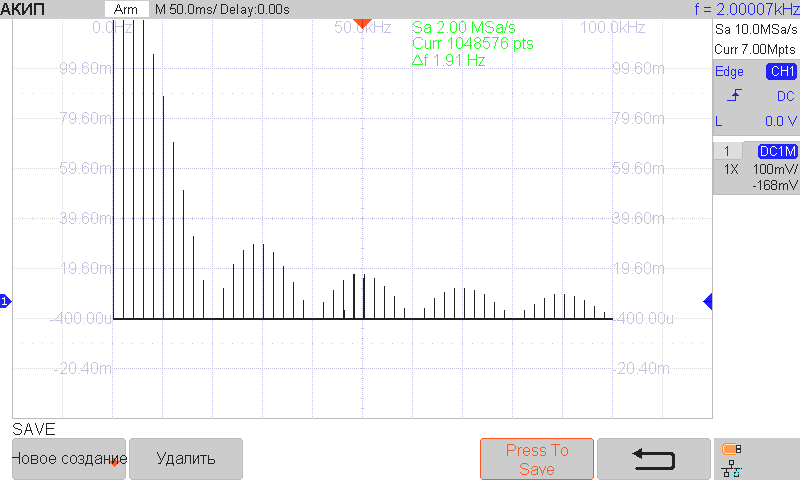
\includegraphics[width=0.5\textwidth]{AKIP0003.png}}}
    \subfloat[$\nu_{\text{повт}} = 2.5$ кГц, $\tau = 50$ мкс]{{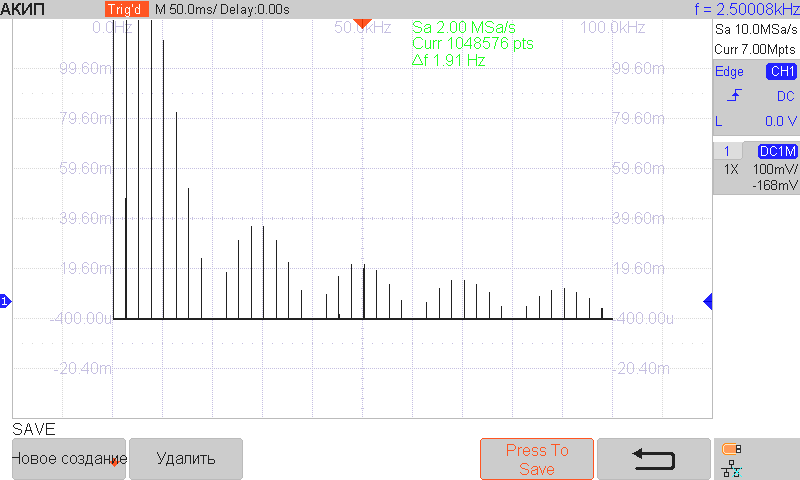
\includegraphics[width=0.5\textwidth]{AKIP0004.png}}}\\
    \end{figure}
\begin{figure}[H]
    \centering
    \subfloat[$\nu_{\text{повт}} = 1$ кГц, $\tau = 60$ мкс]{{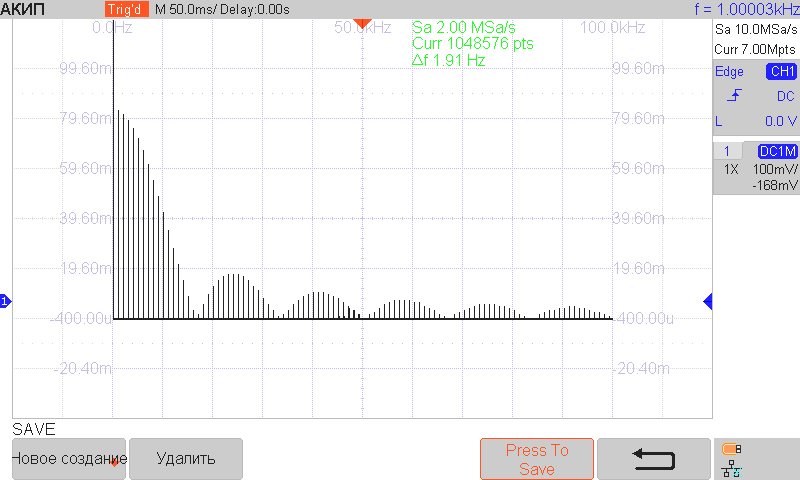
\includegraphics[width=0.5\textwidth]{AKIP0005.png}}}
    \subfloat[$\nu_{\text{повт}} = 1$ кГц, $\tau = 100$ мкс]{{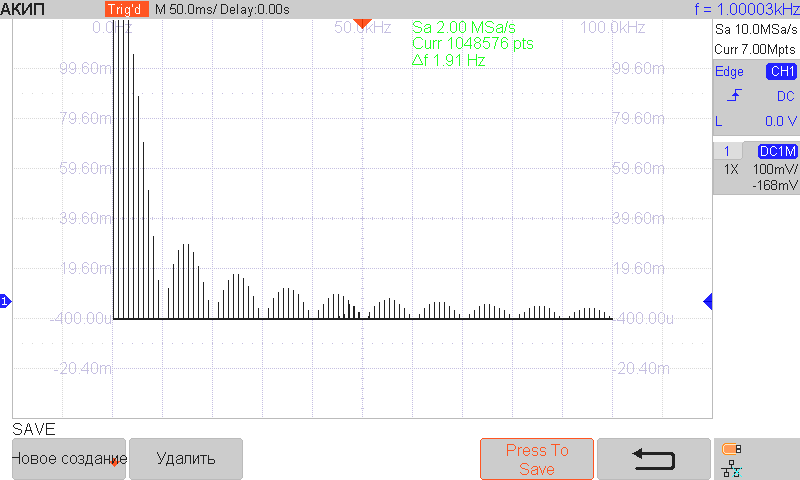
\includegraphics[width=0.5\textwidth]{AKIP0006.png}}}\\
    \end{figure}
\begin{figure}[H]
    \centering
    \subfloat[$\nu_{\text{повт}} = 1$ кГц, $\tau = 150$ мкс]{{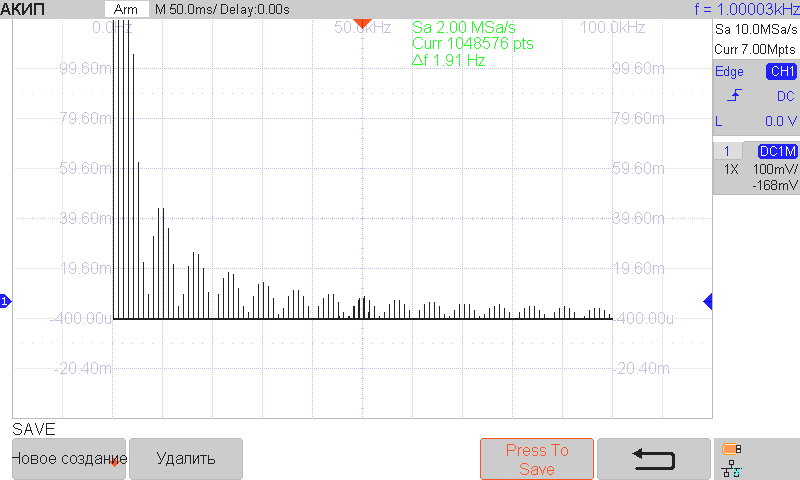
\includegraphics[width=0.5\textwidth]{AKIP0007.png}}}
\end{figure}
\n
Проведя измерения зависимости ширины спектра от $\Delta \nu$, установили связь между $\Delta \nu$ и $\tau$, полученную из формулы $(6)$:
\begin{center}
\begin{tabular}{|c|c|c|c|c|c|c|c|}
\hline
$\tau$, мкс & 50 & 75 & 100 & 125 & 150 & 175 & 200 \\ \hline
$\Delta \nu$, кГц & 19.6 & 13.4 & 9.8 & 8.0 & 6.5 & 5.5 & 4.5 \\ \hline
$1/\tau \cdot 10^3$, с$^{-1}$ & 20 & 13 & 10 & 8 & 7 & 6 & 5 \\ \hline
\end{tabular}
\end{center}
\begin{center}
\fbox{$\Delta \nu \tau = 1,00 \pm 0,02$}
\end{center}
Формула $(6)$ действительно выполняется.

\subsection*{Исследование спектра периодической последовательности цугов}
На экране была получена последовательность цугов с характерными параметрами: $\nu_0 = 50$ кГц, $T = 1$ мс, число периодов в одном импульсе $N = 5$ (длительность импульса $\tau = T/\nu_0 = 100$ мкс).
\begin{figure}[H]
    \centering
    \subfloat[Последовательность цугов]{{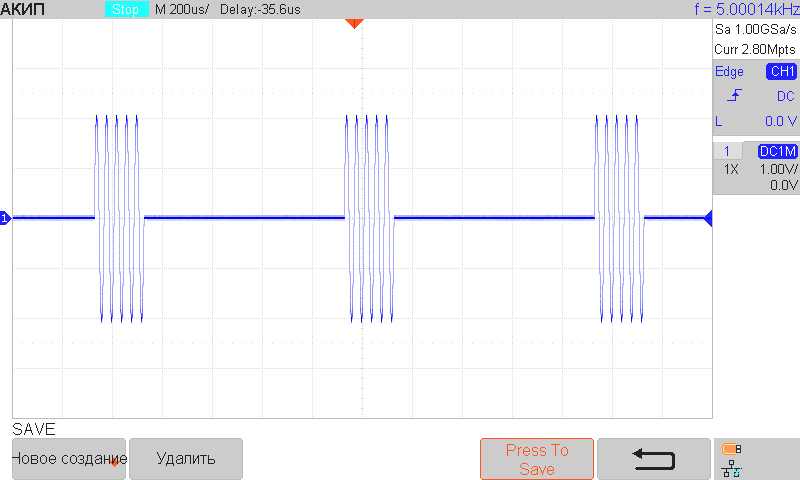
\includegraphics[width=0.5\textwidth]{AKIP0008.png}}}
    \subfloat[Спектр для цугов]{{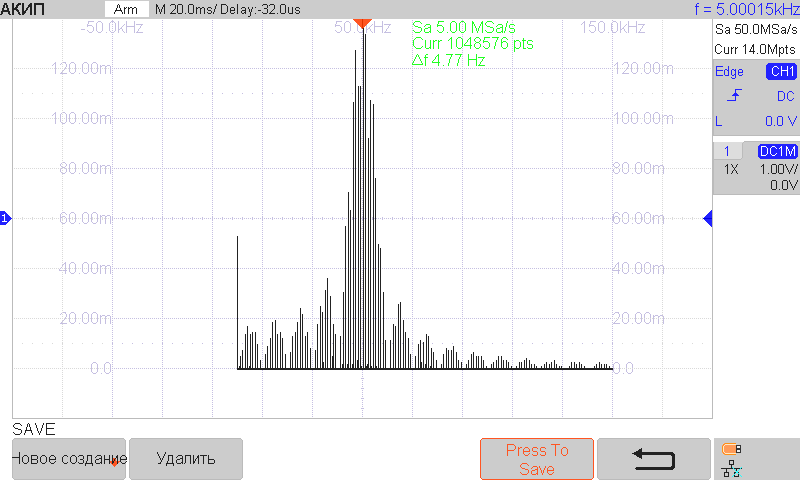
\includegraphics[width=0.5\textwidth]{AKIP0009.png}}}
\end{figure}
\n
Мы изменяли эти параметры по одному и фиксировали результат:
\begin{figure}[H]
    \centering
    \subfloat[$\nu_0 = 50$ кГц, $T = 1$ мс, $N = 10$]{{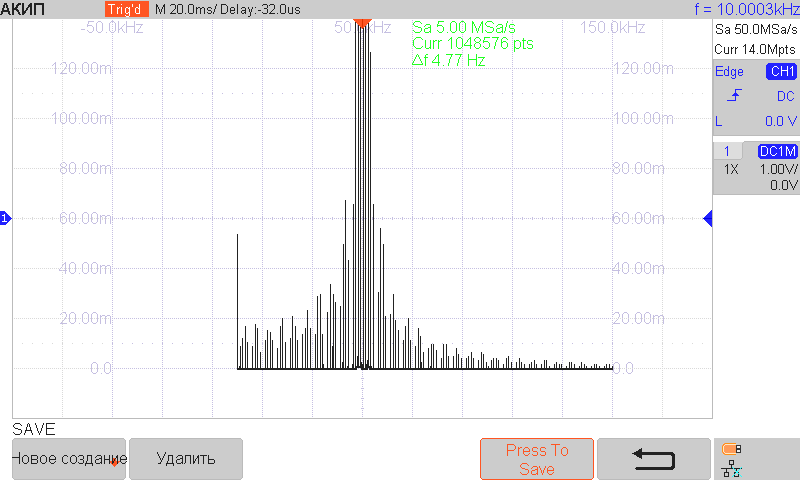
\includegraphics[width=0.5\textwidth]{AKIP0010.png}}}
    \subfloat[$\nu_0 = 50$ кГц, $T = 1$ мс, $N = 15$]{{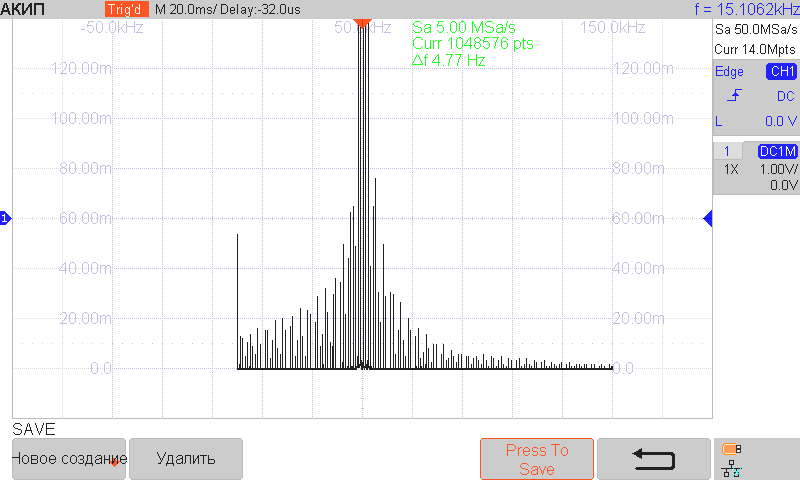
\includegraphics[width=0.5\textwidth]{AKIP0011.png}}}\\
    \end{figure}
    \begin{figure}[H]
    \centering
    \subfloat[$\nu_0 = 50$ кГц, $T = 2.5$ мс, $N = 5$]{{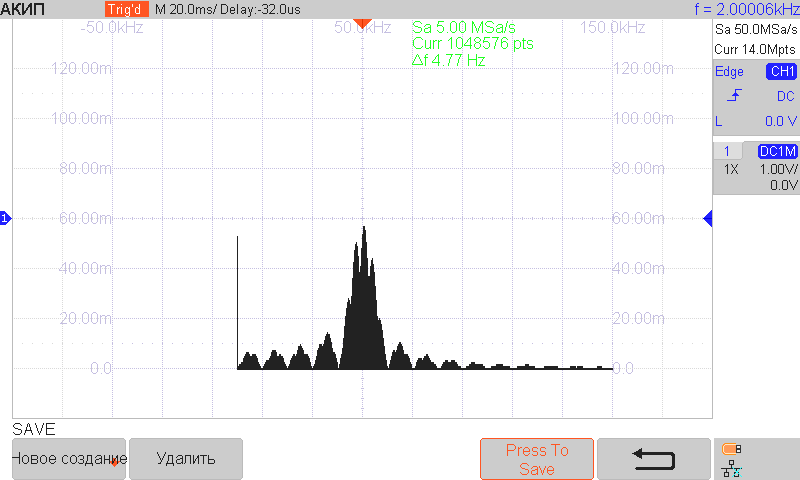
\includegraphics[width=0.5\textwidth]{AKIP0013.png}}}
    \subfloat[$\nu_0 = 50$ кГц, $T = 5$ мс, $N = 5$]{{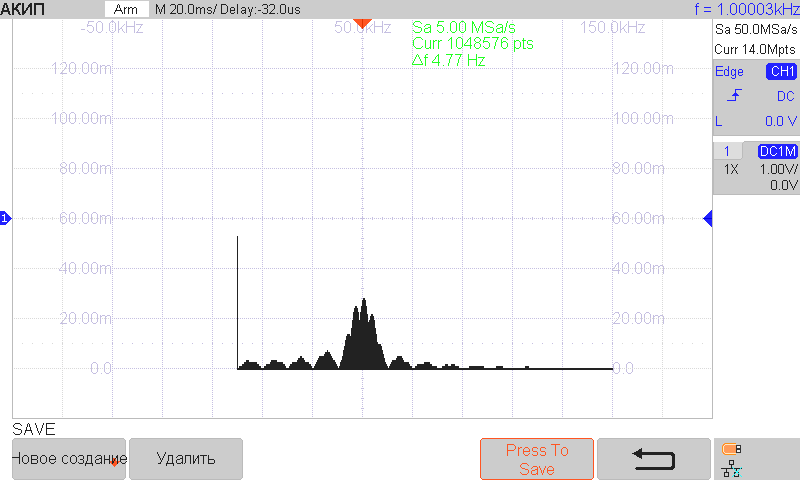
\includegraphics[width=0.5\textwidth]{AKIP0012.png}}}\\
\end{figure}
\begin{figure}[H]
    \centering
    \subfloat[$\nu_0 = 75$ кГц, $T = 1$ мс, $N = 5$]{{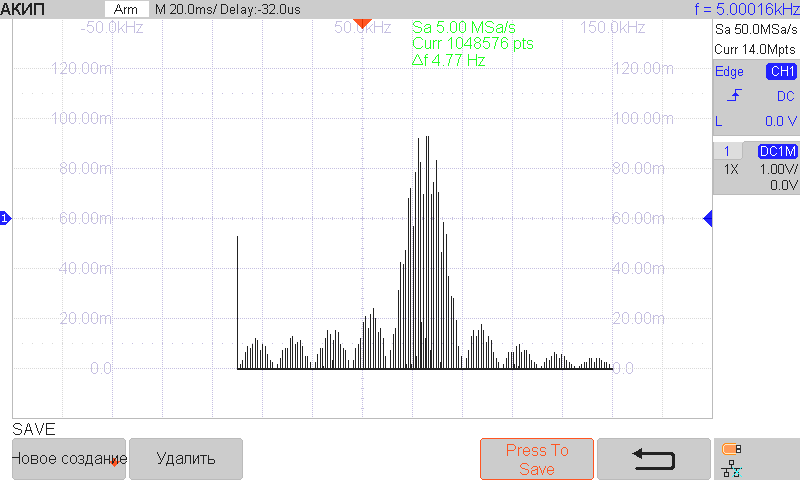
\includegraphics[width=0.5\textwidth]{AKIP0015.png}}}
    \subfloat[$\nu_0 = 100$ кГц, $T = 1$ мс, $N = 5$]{{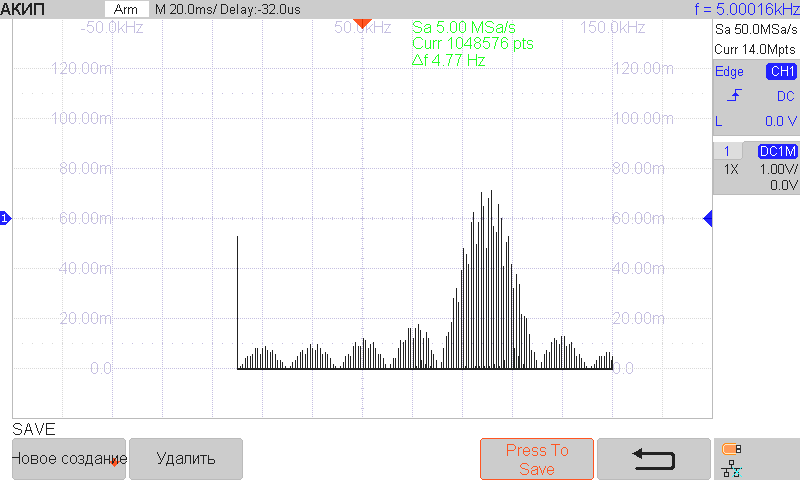
\includegraphics[width=0.5\textwidth]{AKIP0014.png}}}\\
\end{figure}
\n
Далее мы зафиксировали $\nu_0 = 50$ кГц, $N = 5$. Для этих параметров измерили, меняя $T$ ($\nu_{\text{повт}})$, зависимость $\delta \nu$ от $\tau$.
\begin{table}[H]
\centering
\begin{tabular}{|r|r|r|r|r|r|r|}
\hline
$\Delta \nu$, кГц       & 23 & 32 & 35 & 38 & 35 & 45 \\ \hline
$n$                                                   & 42 & 33 & 18 & 13 & 10 &  8 \\ \hline
$\nu_{\text{повт}}$, кГц & 0.5 & 1.0  & 2.0  & 3.0  & 4.0 & 6.0  \\ \hline
\end{tabular}
\end{table}
Итоговое отношение:
\fbox{$\dfrac{\delta \nu}{\nu_{\text{повт}}} = 1,05 \pm 0,08$}
\subsection*{Исследование спектра амплитудно-модулированного сигнала}
На экран выводилась картина амплитудно-модулированного сигнала с характерными параметрами: несущая частота $\nu_0 = 50$ кГц, $\nu_{\text{мод}} = 2$ кГц, глубина модуляции - 50 \% ($m = 0.5$). Картины данного сигнала и его спектра выглядят следующим образом:
\begin{figure}[H]
\centering
 \subfloat[Амплитудно-модулированный сигнал]{{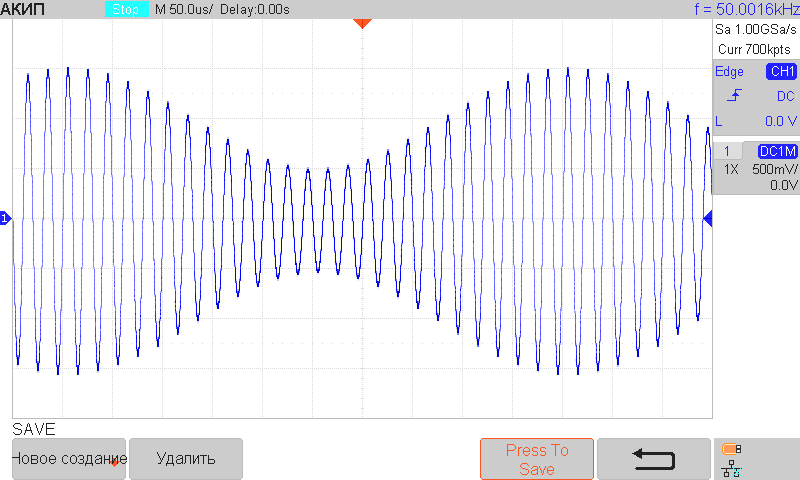
\includegraphics[width = 0.5\textwidth]{AKIP0016.png}}}
    \subfloat[Спектр для $\nu_0 = 50$ кГц, $\nu_{\text{мод}} = 2$ кГц]{{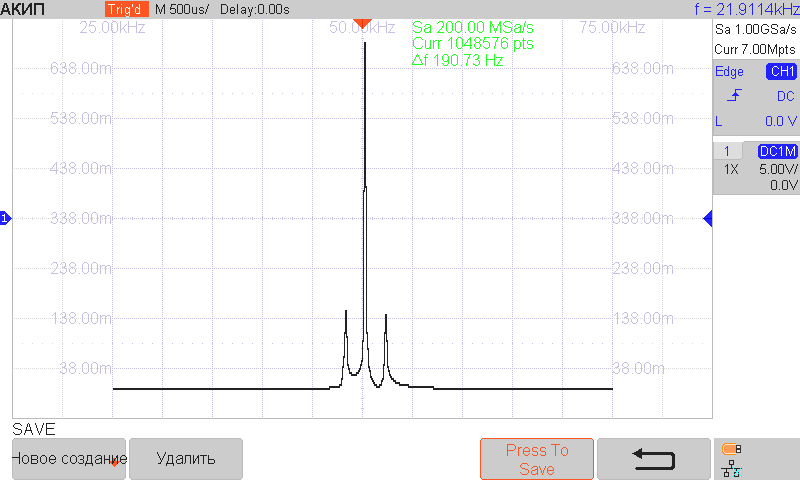
\includegraphics[width=0.5\textwidth]{AKIP0018.png}}}
\end{figure}
\n
Найдем для этого сигнала $A_{max}$ и $A_{min}$ и проверим справедливость формулы $(9)$:
\[A_{max} = 1,52 \text{ В}, \quad A_{min} = 0,48 \text{ В}, \quad m = 0,52\]
\n
Поскольку мы установили глубину модуляции на $0.5$, а из теоретических расчётов получили $0.52$, то видно, что формула $(9)$ верна.
\n\n
Затем мы получили на экране спектр и изменяли параметры сигнала:
\begin{figure}[H]
    \centering
    \subfloat[$\nu_0 = 60$ кГц, $\nu_{\text{мод}} = 2$ кГц]{{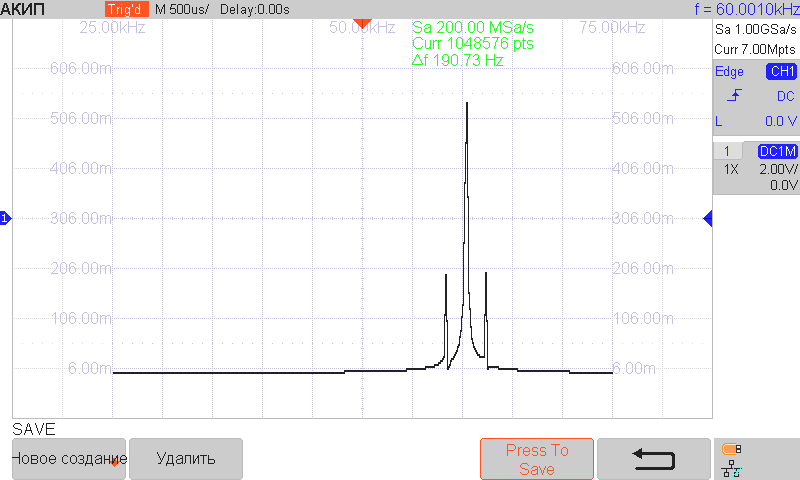
\includegraphics[width=0.5\textwidth]{AKIP0019.png}}}
    \subfloat[$\nu_0 = 70$ кГц, $\nu_{\text{мод}} = 2$ кГц]{{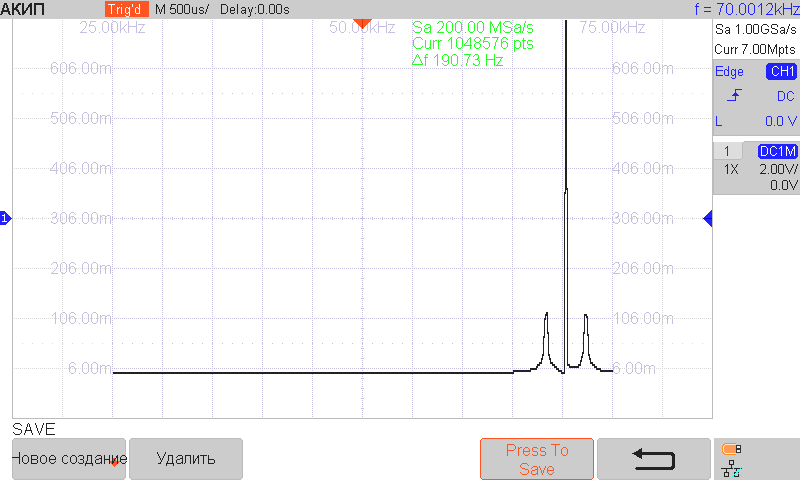
\includegraphics[width=0.5\textwidth]{AKIP0020.png}}}\\
    \end{figure}
    \begin{figure}[H]
    \centering
    \subfloat[$\nu_0 = 50$ кГц, $\nu_{\text{мод}} = 8$ кГц]{{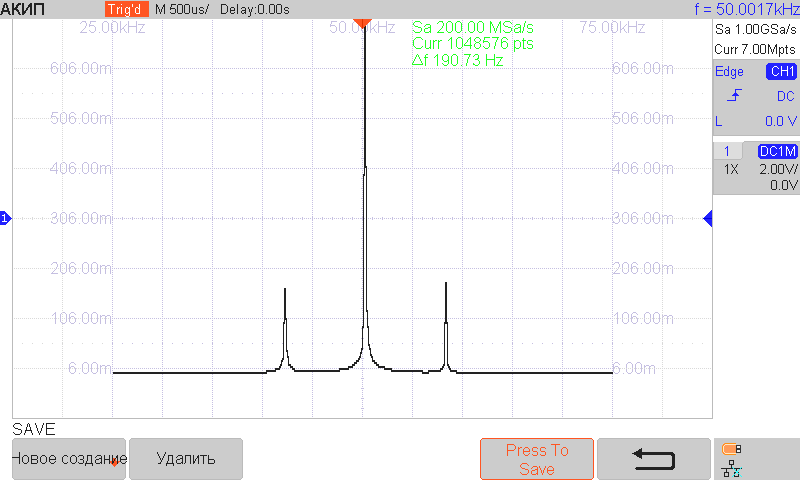
\includegraphics[width=0.5\textwidth]{AKIP0021.png}}}    			\subfloat[$\nu_0 = 50$ кГц, $\nu_{\text{мод}} = 16$ кГц]{{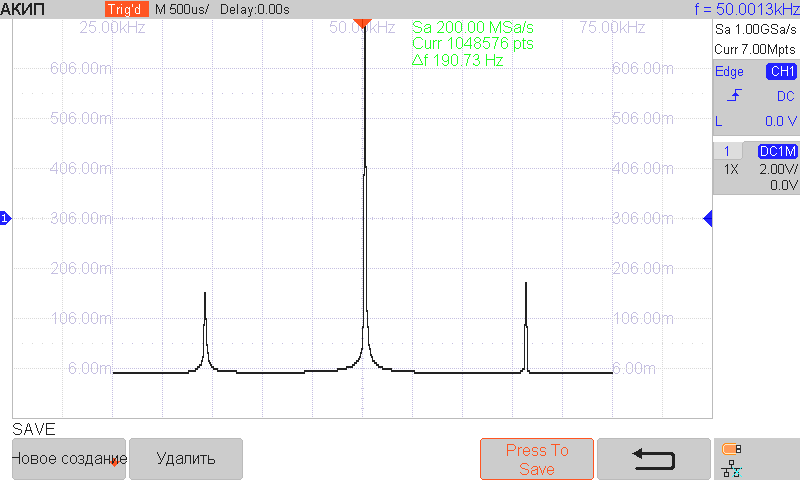
\includegraphics[width=0.5\textwidth]{AKIP0022.png}}}
\end{figure}\n
Из формулы $(10)$ следует, что $a_{\text{осн}} = A_0$, а $a_{\text{бок}} = \dfrac{mA_0}{2}$.
\begin{center}
\begin{tabular}{|c|c|c|c|c|c|}
\hline
$m$, \% & 10 & 25 & 50 & 75 & 100 \\ \hline
$a_{\text{бок}}$, мВ & 360 & 820 & 1660 & 2320 & 3260 \\ \hline
$a_{\text{осн}}$, мВ & 6240 & 6240 & 6240 & 6240 & 6240 \\ \hline
$a_{\text{бок}}/a_{\text{осн}}$ & 0.06 & 0.13 & 0.27 & 0.37 & 0.52 \\ \hline
$a_{\text{бок}}/a_{\text{осн}} \cdot m$, \% & 57.7 & 52.6 & 53.2 & 49.6 & 52.2 \\ \hline
\multicolumn{6}{|c|}{$a_{\text{бок}}/a_{\text{осн}} \cdot m = (53,1 \pm 1,3)$\%} \\ \hline
\end{tabular}
\end{center}
Из $(10)$ имеем $\dfrac{a_{\text{бок}}}{a_{\text{осн}}} \cdot m = 0.5$, что с высокой точностью повторяет наш результат.
\n
\section*{Заключение}
Исследования зависимости ширины спектра периодической последовательности прямоугольных импульсов от длительности отдельного импульса в первой части работы полностью совпали с теоретическими рассчетами. По наклону графика из этой части можно убедиться в соотношении неопределенностей ($\Delta \nu \Delta t \simeq 1$).
\n\n
Исследования зависимости расстояния между ближайшими спектральными компонентами от частоты повторения цугов дали схожие результаты. 
\n\n
В последней части коэффициенты, получаемые в результате исследования зависимости отношения амплитуд спектральных линий синусоидального сигнала, модулированного низкочастотными гармоническими колебаниями, от коэффициента модуляции полностью совпали с теоретически рассчитаными. 

\end{document}
%
%Соберем схему и подготовим приборы к работе, следуя техническому описанию, расположенному на установке.
%
%\subsection*{Часть А}
%B этой части исследуется зависимость ширины спектра периодической последовательности прямоугольных импульсов от длительности отдельного импульса.\n
%Установим на анализаторе спектра режим работы с однократной развёрткой и получим на экране спектр импульсов с параметрами $f_{\text{повт}}=10^{3}$ Гц; $\tau = 100$ мкс; частотный масштаб $m_{x}=5$ кГц/дел.\n
%Проанализируем, как меняется спектр:
%\par a) При увеличении $\tau$ вдвое при неизменном $f_{\text {повт }}=1$ кГц $\Delta \nu$ уменьшается вдвое, а $\delta \nu$ остается неизменным.
%
%\n
%
%\begin{minipage}{0.44\textwidth}
%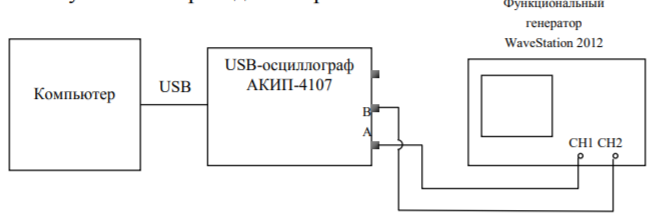
\includegraphics[width=\linewidth]{1.png}
%\begin{center}
%"<Эталонный спектр">
%\end{center}
%\end{minipage}
%\begin{minipage}{0.1\textwidth}
%
%\end{minipage}
%\begin{minipage}{0.44\textwidth}
%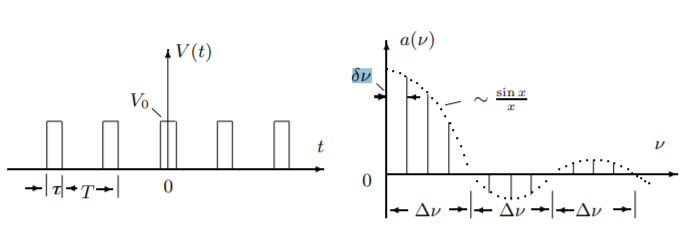
\includegraphics[width=\linewidth]{2.png}
%\begin{center}
%"<Увеличение $\tau$ вдвое">
%\end{center}
%\end{minipage}
%
%\n\n
%
%б) При увеличении $f_{\text {повт }}$ вдвое при неизменном $\tau=100$ мкс $\Delta \nu$ остается неизменным, а $\delta \nu$ увеличивается вдвое. 
%
%\n
%
%\begin{minipage}{0.44\textwidth}
%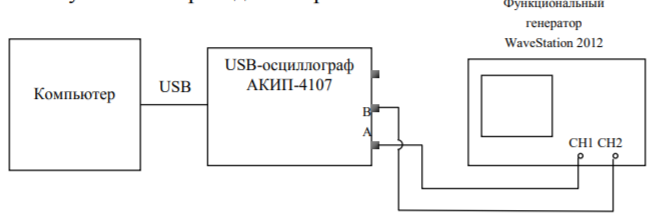
\includegraphics[width=\linewidth]{1.png}
%\begin{center}
%"<Эталонный спектр">
%\end{center}
%\end{minipage}
%\begin{minipage}{0.1\textwidth}
%
%\end{minipage}
%\begin{minipage}{0.44\textwidth}
%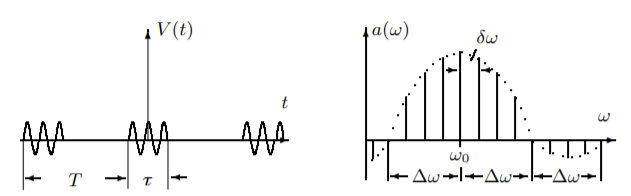
\includegraphics[width=\linewidth]{3.png}
%\begin{center}
%"<Увеличение $f_{повт}$ вдвое">
%\end{center}
%\end{minipage}
%
%\n
%
%Проведем измерения зависимости ширины спектра от длительности импульса $\Delta \nu(\tau)$ при увеличении $\tau$ от 40 до 200 мкс при $f_{\text {повт }}=1$ кГц.\\
%
%\begin{minipage}{0.2\textwidth}
%\begin{tabular}{|c|c|c|c|}
%		\hline
%		$\Delta \nu $  & $ \tau, $ мкс & $ \frac{1}{\tau}, $мкс$^{-1}$ \\ & & $\cdot 10^2 $ \\ 
%		\hline
%25   & 40&2,5\\ 
%		\hline
%17     &60&1,7 \\ 
%		\hline
%13     &  80&1,3 \\ 
%		\hline
%10     &  100&1,0\\ 
%		\hline
% 9     & 120&0,8 \\ 
%		\hline
%7    & 140& 0,7\\ 
%		\hline
%6     &  160&0,6\\ 
%		\hline
%5,4     & 180& 0,6\\ 
%		\hline
%4,9     &200&0,5 \\ 
%		\hline
%	\end{tabular}
%\end{minipage}
%\begin{minipage}{0.09\textwidth}
%\
%\end{minipage}
%\begin{minipage}{0.6\textwidth}
%
%\begin{center}
%		\begin{tikzpicture}[scale = 0.70]
%		\begin{axis}[
%		axis lines = left,
%		ylabel = {$\Delta \nu$},
%		xlabel = {$\tau, $ мкс$^{-1} \cdot 10^2 $},
%		minor grid style={black, line width=0.05pt},
%		major grid style={solid,black, line width=0.3pt},
%		xmin=4, xmax=26,
%		ymin=0.4, ymax=2.6,
%		ymajorgrids = true,
%		xmajorgrids = true,
%		yminorgrids = true,
%		xminorgrids = true,
%		minor tick num = 4
%		]
%		\addplot+[only marks ] plot[error bars/.cd, y dir=both, y explicit]
%		coordinates {
%			(25,2.5)
%			(17,1.67)
%			(13,1.25)
%			(10,1)
%			(9,0.83)
%			(7,0.71)
%			(6,0.63)
%			(5.4,0.56)
%			(4.9,0.5)
%		};
%
%		\addplot[blue, domain=0:30]{0.1*x};
%		\end{axis}
%
%		\end{tikzpicture}
%		
%\end{center}
%\begin{center}
%\ \ \ \ \ \ \ \ \ \ \  График зависимости $\Delta \nu(1 / \tau)$
%\end{center}
%\end{minipage}
%
%\n
%
%По наклону графика можно убедиться в справедливости соотношения неопределённостей.
%
%
%
%\subsection*{Часть Б}
%
%В этой части исследуется зависимость расстояния между ближайшими спектральными компонентами от частоты повторения цугов.
%
%Установим частоту несущей $\nu_{0}=25$ кГц и проанализируем, как изменяется вид спектра: 
%
%a) при увеличении длительности импульса вдвое от $\tau=50$ мкс до $ \tau=100$ мкс для $f_{\text {повт }}=1$ кГц "<ширина"> пиков уменьшается вдвое.
%
%\begin{minipage}{0.44\textwidth}
%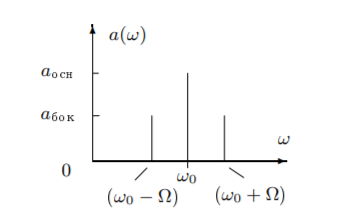
\includegraphics[width=\linewidth]{4.png}
%\begin{center}
%"<Эталонный спектр">
%\end{center}
%\end{minipage}
%\begin{minipage}{0.1\textwidth}
%\end{minipage}
%\begin{minipage}{0.44\textwidth}
%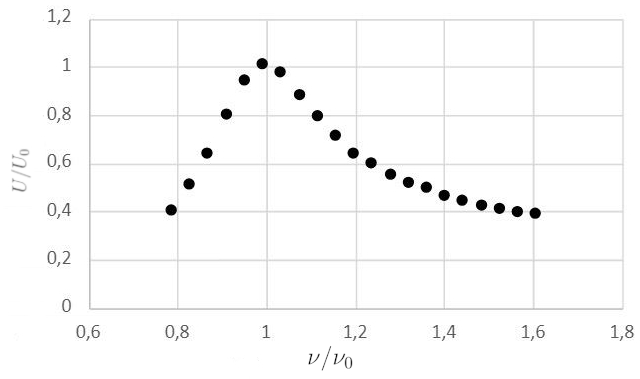
\includegraphics[width=\linewidth]{5.png}
%\begin{center}
%"<Увеличение $\tau$ вдвое">
%\end{center}
%\end{minipage}
%
%\n
%
%б) при изменении частоты несущей: $\nu_{0}=10, 25$ или 40 кГц. изменяется только положение пика.
%
%\begin{minipage}{0.3\textwidth}
%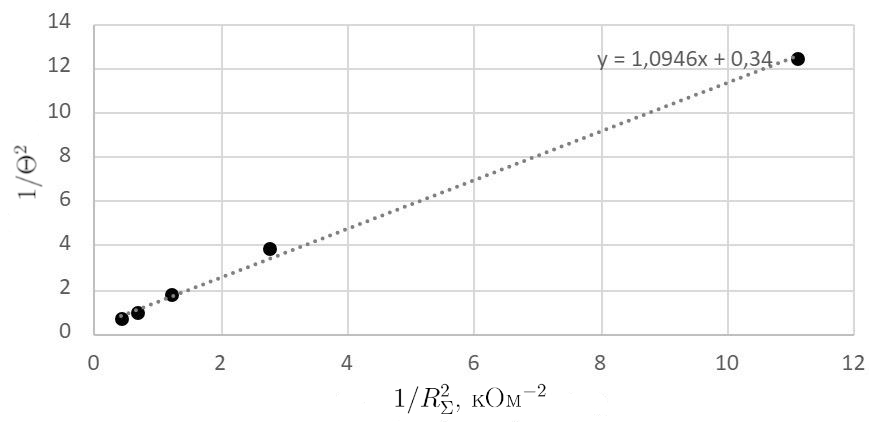
\includegraphics[width=\linewidth]{6.png}
%\begin{center}
%$\nu_{0}=10$ кГц
%\end{center}
%\end{minipage}
%\begin{minipage}{0.05\textwidth}
%\begin{center}
%\end{center}
%\end{minipage}
%\begin{minipage}{0.3\textwidth}
%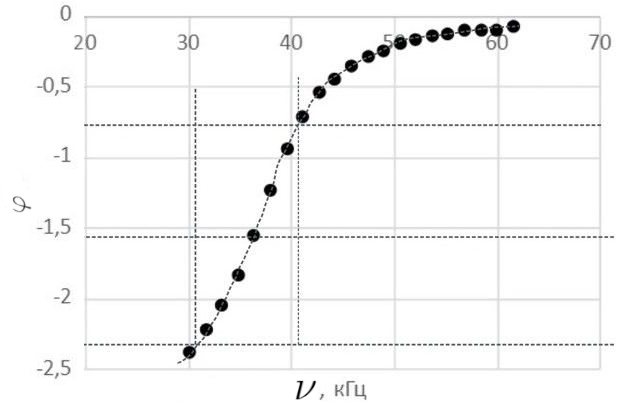
\includegraphics[width=\linewidth]{7.png}
%\begin{center}
%$\nu_{0}=25$ кГц
%\end{center}
%\end{minipage}
%\begin{minipage}{0.05\textwidth}
%\begin{center}
%\end{center}
%\end{minipage}
%\begin{minipage}{0.3\textwidth}
%\includegraphics[width=\linewidth]{8.png}
%\begin{center}
%$\nu_{0}=40$ кГц
%\end{center}
%\end{minipage}
%
%\n
%
%При фиксированной длительности импульсов $\tau=50$ мкс исследуем зависимость расстояния $\delta \nu$ между соседними спектральными компонентами от периода $T$ (частоты повторения импульсов $f_{\text {повт }}$ в диапазоне $0,5-5$ кГц):
%
%\begin{minipage}{0.15\textwidth}
%\begin{tabular}{|c|c|c|}
%		\hline
%		$\delta \nu$   & $f_{\text {повт }}$, \\ & кГц \\ 
%		\hline
%0,5   & 0,5\\ 
%		\hline
%1     &1 \\ 
%		\hline
%2     &  2 \\ 
%		\hline
%4     &  4\\ 
%		\hline
% 5     & 5 \\ 
%		\hline
%	\end{tabular}
%\end{minipage}
%\begin{minipage}{0.04\textwidth}
%\
%\end{minipage}
%\begin{minipage}{0.8\textwidth}
%\vspace{0.8cm}
%\begin{center}
%		\begin{tikzpicture}[scale = 0.8]
%		\begin{axis}[
%		axis lines = left,
%		ylabel = {$\delta \nu$},
%		xlabel = {$f_{\text {повт }}$, кГц},
%		minor grid style={black, line width=0.05pt},
%		major grid style={solid,black, line width=0.3pt},
%		xmin=0, xmax=5.5,
%		ymin=0, ymax=5.5,
%		ymajorgrids = true,
%		xmajorgrids = true,
%		yminorgrids = true,
%		xminorgrids = true,
%		minor tick num = 4
%		]
%		\addplot+[only marks ] plot[error bars/.cd, y dir=both, y explicit]
%		coordinates {
%			(0.5,0.5)
%			(1,1)
%			(2,2)
%			(4,4)
%			(5,5)
%		};
%
%		\addplot[blue, domain=0:30]{x};
%		\end{axis}
%
%		\end{tikzpicture}
%		
%\end{center}
%\begin{center}
%\ \ \ \ \ \ \ \ \ \ \  График зависимости $\delta \nu(f_{\text {повт }})$
%\end{center}
%\end{minipage}
%
%\n\n
%
%По наклону графика можно убедиться в справедливости соотношения неопределённости.
%
%Сравним спектры цугов и прямоугольных импульсов при одинаковых значениях $\tau$ и $T$:
%
%
%\begin{minipage}{0.45\textwidth}
%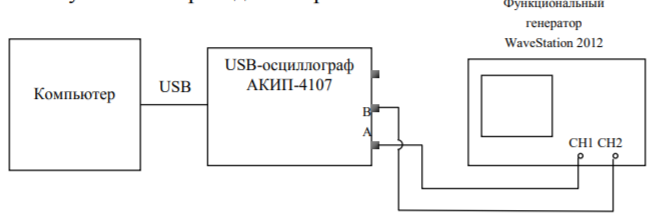
\includegraphics[width=\linewidth]{1.png}\\
%\begin{center}
%Спектр цугов при $\tau = 100 $ мкс $T = 10^{-3} $ c
%\end{center}
%\end{minipage}
%\begin{minipage}{0.05\textwidth}
%\
%\end{minipage}
%\begin{minipage}{0.45\textwidth}
%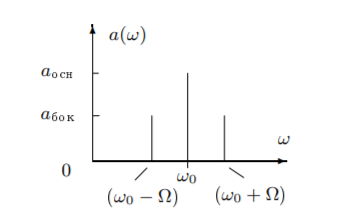
\includegraphics[width=\linewidth]{4.png}\\
%\begin{center}
%Спектр прямоугольных импульсов при $\tau = 100$ мкс и $T = 10^{-3}$ c
%\end{center}
%\end{minipage}
%
%\n\n
%
%Явные отличия - положение пиков и величина амплитуды. 
%
%\subsection{Часть В}
%
%В этой части исследуется зависимость отношения амплитуд спектральных линий синусоидального сигнала, модулированного низкочастотными гармоническими колебаниями, от коэффициента модуляции, который определяется с помощью осциллографа.
%
%Изменяя глубину модуляции, исследуем зависимость отношения амплитуды боковой линии спектра к амплитуде основной линии $\left(a_{\text {бок }} / a_{\text {осн }}\right)$ от глубины модуляции $m ;$ для расчёта глубины модуляции $m$ измерим максимальную $2 A_{\max }$ и минимальную $2 A_{\min }$ амплитуды сигнала на экране осциллографа (см. рис. 6.6 и 6.7). 
%
%\n\n
%
%\begin{minipage}{0.45\textwidth}
%\begin{tabular}{|c|c|c|c|c|}
%		\hline
%	$A_{max}, В \cdot 10 $  & $A_{min}, В \cdot 10 $ &  $ A, В $ & $ m $ \\ 
%		\hline
%   5,55     &  4,50    &   0,2    &     0,104   \\ 
%		\hline
%   6,02     &   4,02   &     0,4  &   0,199     \\ 
%		\hline
%	6,59	        &  3,49    & 0,6      &    0,307    \\ 
%		\hline
%		7,16        & 2,94     &  0,8     &   0,417     \\ 
%		\hline
%7,56		        &    2,55  &    1,0  &   0,495     \\ 
%		\hline
%	8,06	        &   2,02   &     1,2  &    0,599    \\ 
%		\hline
%	8,64	        &    1,49  &    1,4   &    0,705    \\ 
%		\hline
%	9,16	        &     0,98 &    1,6   &     0,806   \\ 
%		\hline
%	9,91	        &   0,56   &     1,8  &     0,893   \\ 
%		\hline
%	1,00	        &    0,17  &    2,0   &    0,966    \\ 
%		\hline
%	\end{tabular}
%\end{minipage}
%\begin{minipage}{0.04\textwidth}
%\
%\end{minipage}
%\begin{minipage}{0.45\textwidth}
%
%\begin{center}
%		\begin{tikzpicture}[scale = 1.0]
%		\begin{axis}[
%		axis lines = left,
%		ylabel = {$m$},
%		xlabel = {$A,\ B$},
%		minor grid style={black, line width=0.05pt},
%		major grid style={solid,black, line width=0.3pt},
%		xmin=0, xmax=2.1,
%		ymin=0, ymax=1.05,
%		ymajorgrids = true,
%		xmajorgrids = true,
%		yminorgrids = true,
%		xminorgrids = true,
%		minor tick num = 4
%		]
%		\addplot+[only marks ] plot[error bars/.cd, y dir=both, y explicit]
%		coordinates {
%			(0.2,0.104)
%			(0.4,0.199)
%			(0.6,0.307)
%			(0.8,0.417)
%			(1,0.495)
%			(1.2,0.599)
%			(1.4,0.705)
%			(1.6,0.806)
%			(1.8,0.893)
%			(2,0.966)
%		};
%
%		\addplot[blue, domain=0:30]{0.5*x};
%		\end{axis}
%
%		\end{tikzpicture}
%		
%\end{center}
%\begin{center}
%\ \ \ \ \ \ \ \ \ \ \  Зависимость $m \ от\ A$
%\end{center}
%\end{minipage}
%\n
%\newpage
%
%Исследуем, как зависит отношнние $a_{\text{бок }} / a_{\mathrm{ocн}}$ от $m$. $A_{осн} = 0.323$ В. 
%
%\n\n
%
%\begin{minipage}{0.45\textwidth}
%\begin{tabular}{|c|c|c|c|c|}
%		\hline
%	$A_{бок}, В \cdot 10  $ & $A_{бок}/A_{осн}$ & $ A, В $ & $m$ \\ 
%		\hline
%   0,016     &  0,048    &   0,2    &     0,104   \\ 
%		\hline
%   0,032     &   0,097   &     0,4  &   0,199     \\ 
%		\hline
%	0,048	        &  0,149    & 0,6      &    0,307    \\ 
%		\hline
%		0,064        & 0,197     &  0,8     &   0,417     \\ 
%		\hline
%0,078		        &   0,246  &    1,0  &   0,495     \\ 
%		\hline
%	0,094	        &   0,289   &     1,2  &    0,599    \\ 
%		\hline
%	0,110	        &    0,341  &    1,4   &    0,705    \\ 
%		\hline
%	0,128	        &     0,396 &    1,6   &     0,806   \\ 
%		\hline
%	0,142	        &   0,440   &     1,8  &     0,893   \\ 
%		\hline
%	0,162	        &    0,500  &    2,0   &    0,966    \\ 
%		\hline
%	\end{tabular}
%\end{minipage}
%\begin{minipage}{0.04\textwidth}
%\n
%\end{minipage}
%\begin{minipage}{0.45\textwidth}
%
%\begin{center}
%		\begin{tikzpicture}[scale = 1.0]
%		\begin{axis}[
%		axis lines = left,
%		ylabel = {$m$},
%		xlabel = {$A_{бок}/A_{осн}$},
%		minor grid style={black, line width=0.05pt},
%		major grid style={solid,black, line width=0.3pt},
%		xmin=0, xmax=0.55,
%		ymin=0, ymax=1.05,
%		ymajorgrids = true,
%		xmajorgrids = true,
%		yminorgrids = true,
%		xminorgrids = true,
%		minor tick num = 4
%		]
%		\addplot+[only marks ] plot[error bars/.cd, y dir=both, y explicit]
%		coordinates {
%			(0.048,0.104)
%			(0.097,0.199)
%			(0.149,0.307)
%			(0.197,0.417)
%			(0.246,0.495)
%			(0.289,0.599)
%			(0.341,0.705)
%			(0.396,0.806)
%			(0.440,0.893)
%			(0.5,0.966)
%		};
%
%		\addplot[blue, domain=0:30]{2*x};
%		\end{axis}
%
%		\end{tikzpicture}
%		
%\end{center}
%\begin{center}
%\ \ \ \ \ \ \ \ \ \ \  Зависимость $m \ от\ A_{бок}/A_{осн}$
%\end{center}
%\end{minipage}
%
%\n\n
%
%
% Угол наклона графика равен 2. 